\documentclass[onecolumn,preprint,superscriptaddress,nofootinbib,notitlepage,10pt,linenumbers]{revtex4-1}
%
%=============================================================================
%\usepackage[margin=1.in]{geometry}
\usepackage{slashed}
\usepackage{graphicx}
\usepackage{amssymb}
\usepackage{mathtools}
\usepackage{bbold}
\usepackage{amssymb,latexsym}
\usepackage{amsmath,amsbsy,bbm}
\usepackage{multirow}
\usepackage[vcentermath]{youngtab}
\usepackage{nicefrac}
\usepackage[perpage]{footmisc}
\usepackage{wrapfig,lipsum,booktabs}
\usepackage{caption}
\usepackage{subcaption}
\usepackage{graphicx}
\usepackage{cjhebrew}

%\usepackage{physics}
\usepackage{floatrow}
\usepackage[dvipsnames]{xcolor} 
%\newfloatcommand{capbtabbox}{table}[][\FBwidth]
%=============================================================================
\newfloatcommand{capbtabbox}{table}[][0.45\textwidth]
%\DefineFNsymbols*{lamportnostar}[math]{\dagger\ddagger\S\P\|{\dagger\dagger}{\ddagger\ddagger}}
%\setfnsymbol{lamportnostar}
%\renewcommand\thefootnote{\fnsymbol{footnote}}
%=============================================================================
\newcommand{\es}{1\text{\scriptsize s}}
\newcommand{\zs}{2\text{\scriptsize s}}
\newcommand*{\mprime}{^{\prime}\mkern-1.2mu}
\newcommand{\largescale}{\ensuremath{\Lambda_\text{Hi}}}
\newcommand{\lc}{\ensuremath{\Lambda_c}}
\newcommand{\fm}{\ensuremath{\,\text{fm}^{-1}}}
\newcommand{\abb}{\mbox{\ensuremath{A\oplus 1}}}
\newcommand{\red}[1]{\textcolor{red}{#1}} 
\newcommand{\green}[1]{\textcolor{green}{#1}} 
\newcommand{\blue}[1]{\textcolor{blue}{#1}} 
\newcommand{\lec}{C^\Lambda}
\newcommand{\led}{D^\Lambda}
\newcommand{\ddrei}[1]{\delta_{\tiny \Lambda}^{(3)}\!\big(#1\big)}
\newcommand{\wrt}{\textit{w.r.t.}~}
\newcommand{\etc}{\textit{etc.}~}
\newcommand{\eg}{\textit{e.g.}~}
\newcommand{\ie}{\textit{i.e.}~}
\newcommand{\viz}{\textit{viz.}~}
\newcommand{\eftnopi}{\mbox{EFT$(\not \! \pi)$}}
\newcommand{\ve}[1]{\ensuremath{\boldsymbol{#1}}}
\newcommand{\rms}[1]{\ensuremath{\langle r(#1)\rangle}}
\newcommand{\ls}{\ve{L}\cdot\ve{S}}
\newcommand{\be}{\begin{equation}}
\newcommand{\ee}{\end{equation}}
\newcommand{\bra}{\big\langle}
\newcommand{\ket}{\big\rangle}
\newcommand{\hl}{\big\vert}
\newcommand{\vcl}[1]{\ensuremath{\bar{\boldsymbol{r}}_\text{\tiny #1}}}
\newcommand{\vsp}[1]{\ensuremath{\boldsymbol{r}}_\text{\tiny #1}}
\newcommand{\la}{\label}
\newcommand{\Pe}{\text{\cjRL{p|}}}
\newcommand{\figref}[1]{fig.~\ref{#1}}
\newcommand{\tabref}[1]{table~\ref{#1}}
\newcommand{\ccite}[1]{Ref.~\cite{#1}}
%\newcommand{\bra}[1] {\left\langle~#1~\right|}
%\newcommand{\ket}[1] {\left|~#1~\right\rangle}
\newcommand{\bet}[1] {\left|#1\right|}
\newcommand{\overlap}[2] {\left\langle\,#1\,\left|\,#2\,\right.\right\rangle}
\newcommand{\me}[3] {\left\langle\,#1\,\left|\left.\,#2\,\right|\,#3\,\right.\right\rangle}
\newcommand{\redme}[3] {\left\langle\,#1\,\middle|\right|\,#2\,\left|\middle|\,#3\,\right\rangle}

\definecolor{blue}{HTML}{4169E1}
\definecolor{red}{HTML}{DC143C}
\definecolor{green}{HTML}{2E8B57}
\definecolor{mandarin}{HTML}{FF9933}

\newcommand{\MPV}[1]{\textcolor{purple}{#1}}
\newcommand{\LC}[1]{\textcolor{mandarin}{#1}}
\newcommand{\JK}[1]{\textcolor{green}{#1}}
\newcommand{\note}[1]{\textbf{\textcolor{gray}{#1}}}
%=============================================================================
\usepackage[normalem]{ulem}

\DefineFNsymbols*{lamportnostar}[math]{\dagger\ddagger\S\P\|{\dagger\dagger}{\ddagger\ddagger}}
\setfnsymbol{lamportnostar}
\renewcommand\thefootnote{\fnsymbol{footnote}}
\let\endtitlepage\relax

\begin{document}

\title{Universality of the multi-channel 4-body scattering system}
\author{Jean Luc Picard}
\email{jeanluc@1701.ncc}
\affiliation{Starfleet Academy, Fort Baker, San Francisco, Earth}
\date{\today}

\begin{abstract}
We investigate the scattering system of 4 equal-mass quantum particles at energies
where rearrangement channels are open. The interactions are renormalized to capture
the essence of the pertinent nuclear 2-neutron, 2-proton system. A full
treatment of the Coulomb interaction is included.

The quantity of most practical interest, namely the coupling between the deuteron-deuteron
and the ${}^3$H-proton/${}^3$He-neutron channels, is subjected to a sensitivity analysis
with respect to distorted, \ie, screened Coulomb repulsion between the two protons.
\end{abstract}

\maketitle

\section{Few is more}

Na\"ively, one expects the probability of a neutron (proton) transfer from a projectile deuteron onto a target neutron
and the ensuing ejection of a triton (3-helium) plus a proton (neutron) to be strongly correlated with the
efficiency of a device which is able to harvest the energy thereby released. Any mechanism which increases this probability
is thus of practical interest.

As quantified in \figref{fig.dd-phases}, the strong nuclear force and the point-Coulomb repulsion between protons
do not yield a strong coupling between the deuteron-deuteron and the 3-1 fragment channels (fat red line, bottom panel).

the scattering process is parametrized via a 3-channel S-matrix:
\be
\la{eq.sm}
S_{ij}=\me{a\,L_a\,S_a}{\hat{S}^{J^\pi}}{b\,L_b\,S_b}=\eta_{ij}\,e^{2i\delta}
\;\;,\qquad
\ee

and the almost decoupled d-d channel is encoded in $\eta_{dd}\approx 1$. Although, the Coulomb repulsion between protons
provides a heuristic argument for this weak coupling, the comparison to the relatively strong coupling between the two 3-1
fragmentations seems to defy the argument as an equally strong force keeps the proton out of 3-helium.

%--
\begin{figure}[tb]
\centerline{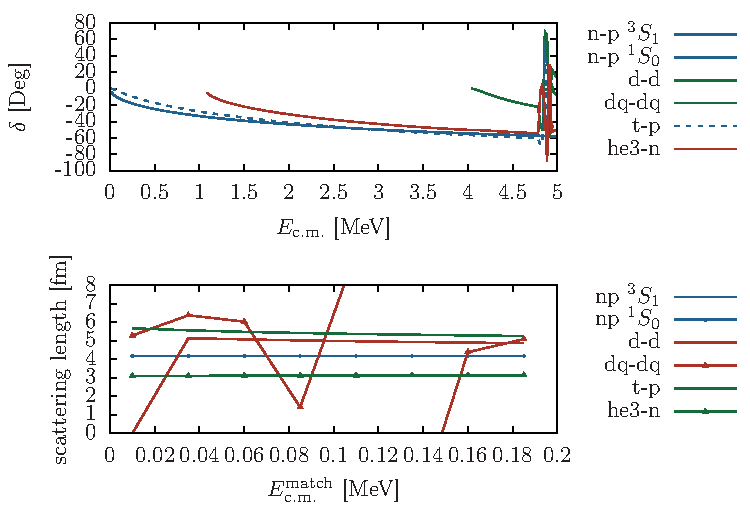
\includegraphics{/home/kirscher/kette_repo/limit_cycles/systems/4/0p_phases.pdf}}
\caption{\label{fig.dd-phases} Energy dependence of phase shifts which parameterize the coupled channel
nnpp system in the ${}^1S_0$ $\alpha$ channel~\eqref{eq.sm}.
}
\end{figure}
%--

\bibliography{refs}

\end{document}